\documentclass{article} 

\usepackage{amsmath}
\usepackage{amssymb}
\usepackage[margin=1.0in]{geometry}
\usepackage{hyperref}
\usepackage{graphicx}
\usepackage{pgfplots}
\usepackage{siunitx}
\usepackage[notquote]{hanging}
\pgfplotsset{compat=newest}

\providecommand{\abs}[1]{\lvert#1\rvert}
\providecommand{\norm}[1]{\lVert#1\rVert}

\title{An algorithm for determining the composition of a musical chord using 
	Fourier transformations}

\author{Marko Vejnovi\'{c}}

\begin{document}
\maketitle

\section{Rationale}
\paragraph*{}
As someone who is interested in signals, music and mathematics it was obvious 
for me that I wanted my mathematics internal assessment to be related to 
music. Although I have known of and used the Fourier transformations before, I 
have never used Fourier transformations to find individual notes in sounds. I 
decided, therefore, to try and identify chords using Fourier transformations, 
and try to find which are the composing notes of a chord.

\section{Introduction}

\paragraph*{}
Even now, in the 21st century, an algorithm for identifying tones in music 
does not exist\footnote{Trained models are able to identify tones, however, 
there doesn't exist a single untrained algorithm which can achieve this.}. 
Research has been done which does allow simple chord progressions to be 
identified, but complex progressions remain a mystery.

\paragraph*{}
The likes of Hausner, Kurnia and of course, Wang, have developed algorithms 
which present themselves as being promising. Although currently, simple, with 
the exception of Wang's, these algorithms are powerful enough to follow chord 
progressions. However, with advancements in the field, it is likely that these 
algorithms would improve to a point where they could follow highly complex, 
highly noisy melodies, for example, in music like jazz and rock.

\paragraph*{}
The research goal of this paper is to create a simple algorithm with decent 
performance which allows for recognizing chords and the individual tones that 
make them up. This simple algorithm could prove useful as a piece of a bigger 
algorithm for identifying chord progressions in songs.

\subsection{Musical background}

\paragraph*{}
A chord is a musical unit in which three or more tones are played 
simultaneously (Benward, and Saker). The most simple chords are 
\textit{triads}, as they are composed of only three tones. Although they are 
modeled by three composing sine waves (for example, the $C$ major chord is 
$f_{C_4maj} (t) = sin(41.63t) + sin(52.46t) + sin(62.39t)$), it is very 
important to note that actual musical instruments do not produce sine waves, 
as there are physical events that prevent this - reverb\footnote{Reverberation 
is the effect of reflecting sound waves. When sound waves reflect off of 
surfaces many of them build up and then decay as they become absorbed (Valente 
et al.). It is what allows us to discern from big halls to small studios when 
hearing audio.}, distortion\footnote{Distortion is most easily modeled as 
clipping. If a signal function is defined as $f(t) = A(a) sin(\omega t)$ then 
clipping will, for example, occur when:
$$A(a) = 
\begin{cases}
	-4	& \text{when }a < -4 \\
	a	& \text{when }-4 < a < 4 \\
	4	& \text{when }a > 4 \\
\end{cases}
$$
This is an example of hard clipping, and is the simplest example, but other, 
more complicated examples exist.}, harmonic series\footnote{The harmonic 
series is the result of multiple parts of a vibrating body vibrating 
themselves (Benward, and Saker). A tone, therefore, is not composed of only 
one sine wave, but multiple sine waves of varying amplitudes. Usually, the 
longest harmonic is the strongest.}, etc.

\paragraph*{}
Another major issue stands - the timbre of a musical instrument. 
\textit{Timbre} does not have a clear-cut definition as it is quite abstract, 
but can be thought of as the color of the sound a musical instrument produces, 
ie. it is the property (or, rather \textit{properties}) that allow us to 
discern musical instruments from one another.

\paragraph*{}
All of these effects hinder the possibility of easily and effectively fitting 
a function using the least squares method. To find the individual frequencies 
composing a chord, it is necessary to convert the chord signal from the time 
domain to the frequency domain. For this, the \textit{Fourier transformation} 
is used.

\subsection{Fourier transformation}

\paragraph*{}
To understand the Fourier transformation, a definition of what the Fourier 
series is necessary.

\subsubsection{Fourier series}

\paragraph*{}
The Fourier series is a method of representing arbitrary periodic functions as 
a sum of simple sine and cosine functions. A method for deriving it follows.

\paragraph*{}
Suppose an even function such as the one graphed in figure 
\ref{fig:odd-arb-func} exists.
\begin{figure}[ht]
	\centering
	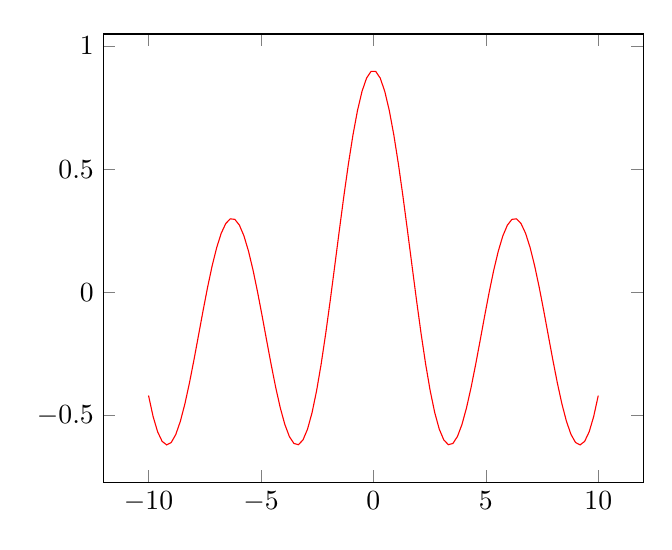
\begin{tikzpicture}
		\begin{axis}
			\addplot[
				color=red,
				domain=-10:10,
				samples=100
			]{0.3 * cos(deg(0.5 * x)) + 0.6 * cos(deg(x))};
		\end{axis}
	\end{tikzpicture}
	\caption{An arbitrary even function}
	\label{fig:odd-arb-func}
\end{figure}

The premise is that it is possible to express this function as a sum of cosine 
waves:
$$f(t) = \sum^{\infty}_{n=0}a_n \cos(2 \pi n t)$$

Note that $n$ is the frequency of the wave in $\si{Hz}$. This derivation will 
employ $\si{Hz}$, however, no difference does it pose to use a radial frequency
either.

However, from this premise, it is necessary to calculate the values of $a_n$'s. 
This problem is solved in the following manner:

\paragraph*{}
Both sides are multiplied by $\cos(2 \pi m t)$:
$$f(t) \cos(2 \pi m t) = \sum^{\infty}_{n=0}b_n \cos(2 \pi n t) \cos(2 \pi m t)$$
Next, both sides are integrated over one period of the function, and the 
trigonometric identity of the product of cosines is employed:
\begin{equation}
	\begin{aligned}
		\int_{T} f(t) \cos(2 \pi m t) dt &= 
		\int_{T} \sum^{\infty}_{n=0} a_n \cos(2 \pi n t) \cos(2 \pi m t) dt \\
		&= \sum^{\infty}_{n=0} a_n \int_{T} \cos(2 \pi n t) \cos(2 \pi m t) dt \\
		&= \frac{1}{2} \sum^{\infty}_{n=0} a_n \int_{T} \Big(\cos \big( (m + n) 2 \pi t \big) + \cos \big( (m - n) 2 \pi t \big) \Big) dt \\
	\end{aligned}
	\label{eqn:fourier-series-1}
\end{equation}
Suppose $m \geq 0$ (this is possible to suppose because $m$ is arbitrary, and 
more importantly, it is physically impossible for frequency to be negative). 
From this it follows that $\cos \big( (m + n) 2 \pi t \big)$ has $m + n$ 
oscillations in a single period $T$, and consequently, $m + n$ oscillations in 
the integration interval. Since this is true, when this function is integrated, 
the result is $0$\footnote{The proof for this is trivial, however, it is 
published by a third party online and is available to the reader at the 
following link: \url{http://planetmath.org/integraloveraperiodinterval}.}. 
Equation \ref{eqn:fourier-series-1} is then simplified to:
\begin{equation}
	\begin{aligned}
		\int_{T} f(t) \cos(2 \pi m t) dt &=
		\frac{1}{2} \sum^{\infty}_{n=0} a_n \bigg(\int_{T} \cos( (m + n) 2 \pi t) dt + 
		\int_{T} \cos( (m - n) 2 \pi t) dt \bigg) \\
		&= \frac{1}{2} \sum^{\infty}_{n=0} a_n \int_{T} \cos( (m - n) 2 \pi t) dt
	\end{aligned}
	\label{eqn:fourier-series-2}
\end{equation}
Since the cosine function is even, in a single period $T$ (the integration 
interval - from $-\frac{T}{2}$ to $\frac{T}{2}$) the following is true:
$$\cos( (m - n) 2 \pi t) = \cos( (n - m) 2 \pi t)$$
When $m = n$:
$$\cos( (m - n) 2 \pi t) = \cos(0) = 1$$

Due to the orthogonality of sines and cosines\footnote{The orthogonality of 
	sines and cosines is outside of the scope of this paper, but in a nutshell,
	it is the property of sines and cosines which states that:
	\[
		\int_{-\frac{T}{2}}^{\frac{T}{2}} \cos \bigg(\frac{(n + m) \pi}{T} t \bigg) + \cos \bigg(\frac{(n - m) \pi}{T} t \bigg) dt = 0 \text{ when } m \neq n
	\]
This paper considers it as a premise.} it follows that:
\[
	\int_{T} \cos( (m - n) 2 \pi t) = 
	\begin{cases}
		\int_{T} \cos ( (m -n) 2 \pi t) dt = 0 & \text{when } m \neq n \\
		\int_{T} 1 \cdot dt = T & \text{when } m = n
	\end{cases}
\]
It is key to note that:
$$\forall (0 < m < \infty, 0 < n < \infty \land m \neq n) \rightarrow
\int_{T} cos( (m - n) 2 \pi t) dt = 0$$
From this it follows that the whole summation in equation 
\ref{eqn:fourier-series-2} can be reduced to the case when $m = n$:
$$\int_T = f(t) \cos(m 2 \pi t) dt = \frac{1}{2} a_m T$$
To get $a_m$ is trivial:
\begin{equation*}
	a_m = \frac{2}{T} \int_T f(t) \cos(m 2 \pi t) dt
\end{equation*}
Finally, replacing $m$ with $n$ we get:
\begin{equation}
	a_n = \frac{2}{T} \int_T f(t) \cos(m 2 \pi t) dt
	\label{eqn:fourier-series-amp}
\end{equation}

However, the case of $m = 0$ is not considered. This case gives the $y$ axis 
offset $a_0$. Substituting with $m = 0$ in equation \ref{eqn:fourier-series-1}, 
we get:
$$
\begin{aligned}
\int_{T} f(t) \cos(2 \pi m t) dt &= 
\sum^{\infty}_{n=0} a_n \int_{T} \cos(2 \pi n t) \cos(2 \pi m t) dt \\ 
\int_T f(t) \cos(0) dt &= \sum^{\infty}_{n=0} a_n \int_T \cos(2 \pi n t) \cos(0) dt \\
\int_T f(t) dt &= \sum^{\infty}_{n=0} a_n \int_T \cos(2 \pi n t) dt \\
\int_T f(t) dt &= T a_0
\end{aligned}$$
This gives the final result for the $y$ axis offset:
\begin{equation}
	a_0 = \frac{1}{T} \int_T f(t) dt
	\label{eqn:fourier-series-yoffset}
\end{equation}
This result is coincidentally intuitively the average of all of the $y$ values 
of the points of the function in a single period.

Odd functions are represented in a similar manner:
$$f_o(t) = \sum^{\infty}_{n=1} b_n \sin(2 \pi n t)$$
The coefficients $b_n$ are, then:
$$b_n = \frac{2}{T}\int_T f_o(t) \sin(2 \pi n t) dt$$
As the derivation is quite similar to the one for the even function, it has 
been omitted.

Since any arbitrary function $f(t)$ can be represented as a sum of odd and even 
functions:
$$f_o(t) = \frac{1}{2}(f(t) - f(-t))$$
$$f_e(t) = \frac{1}{2}(f(t) + f(-t))$$
$$f(t) = f_o(t) + f_e(t)$$
The Fourier series' components can be applied:
$$f(t) = a_0 + \sum^{\infty}_{n=1} (a_n \cos(2 \pi n t) + b_n \sin(2 \pi n t))$$
with the coefficients being:
$$a_0 = \frac{1}{T} \int_T f(t) dt$$
$$a_n = \frac{2}{T} \int_T f(t) \cos(2 \pi n t) dt, n \neq 0$$
$$b_n = \frac{2}{T} \int_T f(t) \sin(2 \pi n t) dt$$

It is possible to express the Fourier series in its complex form, using 
Euler's formulas:
$$cos \phi = \frac{e^{i\phi} + e^{-i\phi}}{2}$$
$$sin \phi = \frac{e^{i\phi} - e^{-i\phi}}{2i}$$
\begin{equation*}
	\begin{aligned}
		f(t) &=
		a_0 + \sum^{\infty}_{n=1}(a_n \cos(2 \pi n t) + b_n \sin(2 \pi n t)) \\
		& = a_0 + \sum^{\infty}_{n=1}\Big(
		a_n \frac{e^{i 2 \pi n t} + e^{-i 2 \pi n t}}{2} + 
		b_n \frac{e^{i 2 \pi n t} - e^{-i 2 \pi n t}}{2i}\Big) \\
		&= a_0 + \sum^{\infty}_{n=1} \frac{a_n - ib_n}{2}e^{2 \pi n t} +
		\sum^{\infty}_{n=1} \frac{a_n + ib_n}{2} e^{-2 \pi n t}
	\end{aligned}
\end{equation*}

Let us know define $c_n$ as 
$$c_n = \frac{a_n - i b_n}{2}$$

This gives the complex Fourier series:
\begin{equation*}
	f(t) = \sum^{\infty}_{n = - \infty} c_n e^{i 2 \pi t}
\end{equation*}
This is referred to as the \textit{synthesis} equation.

From this it follows that $c_n$, the complex Fourier coefficient, is:
\begin{equation*}
	\begin{aligned}
		c_n &= 
		\frac{1}{2} \cdot \bigg( \frac{2}{T} \int_T f(t) \cos(2 \pi n t) dt - 
		i \frac{2}{T} \int_T f(t) \sin(2 \pi n t) dt \bigg) \\
		&= \frac{1}{T} \int_T f(t) \cos(2 \pi n t) - i f(t) \sin(2 \pi n t) dt \\
		&= \frac{1}{T} \int_T f(t) \bigg( 
			\frac{e^{i 2 \pi n t} + e^{-i 2 \pi n t}}{2} - 
		i \frac{e^{i 2 \pi n t} - e^{-i 2 \pi n t}}{2i} \bigg) \\
		&= \frac{1}{T} \int_T f(t) \frac{2 e^{i 2 \pi n t}}{2} dt \\
		c_n &= \frac{1}{T} \int_T f(t) e^{-i 2 \pi n t} dt
	\end{aligned}
\end{equation*}
This is referred to as the \textit{analysis} equation. This equation gives 
spectral lines for a frequency $n$. Note that it is not continuous.

\subsection{The Fourier transformation}

\paragraph*{}
The Fourier transformation can be thought of as a continuous version of the 
Fourier series:
$$\hat{f} (t) = \int^{\infty}_{-\infty} f(t) e^{-i 2 \pi \nu t} dt$$

\paragraph*{}
Let the Fourier transformation be defined as the limit of the analysis 
formula of the Fourier series as $T$ approaches infinity:
$$\hat{f} (t) = \lim_{T \rightarrow \infty} c_n = \lim_{T \rightarrow \infty} 
\int_{-T / 2}^{T / 2} f(t) e^{-i 2 \pi n t} dt$$
Note the factor $\frac{1}{T}$ is completely ignored, due to the fact that 
$\lim_{n \rightarrow \infty} \frac{1}{n} = 0$, which would ruin the function. 
This is far more relevant when doing the inverse Fourier transformation, 
however the inverse Fourier transformation is outside of the scope of this 
paper and therefore is not explored. The limit makes the spectral lines come 
closer, creating the final equation:
$$\hat{f} (t) = \int_{-\infty}^{\infty} f(t) e^{-i 2 \pi \nu t} dt$$
The power of this equation lies in the fact that it gives a continuous 
function showing the frequencies of a \textit{non-periodic} signal. In turn, 
it has practical applications in converting a signal from the time domain to 
the frequency domain.

\section{The chord identification algorithm}

\paragraph*{} 
Given an input signal such as the one given in figure \ref{fig:input-signal}, 
the algorithm operates in %TODO
distinct stages.
\begin{figure}[ht] 
	\centering
	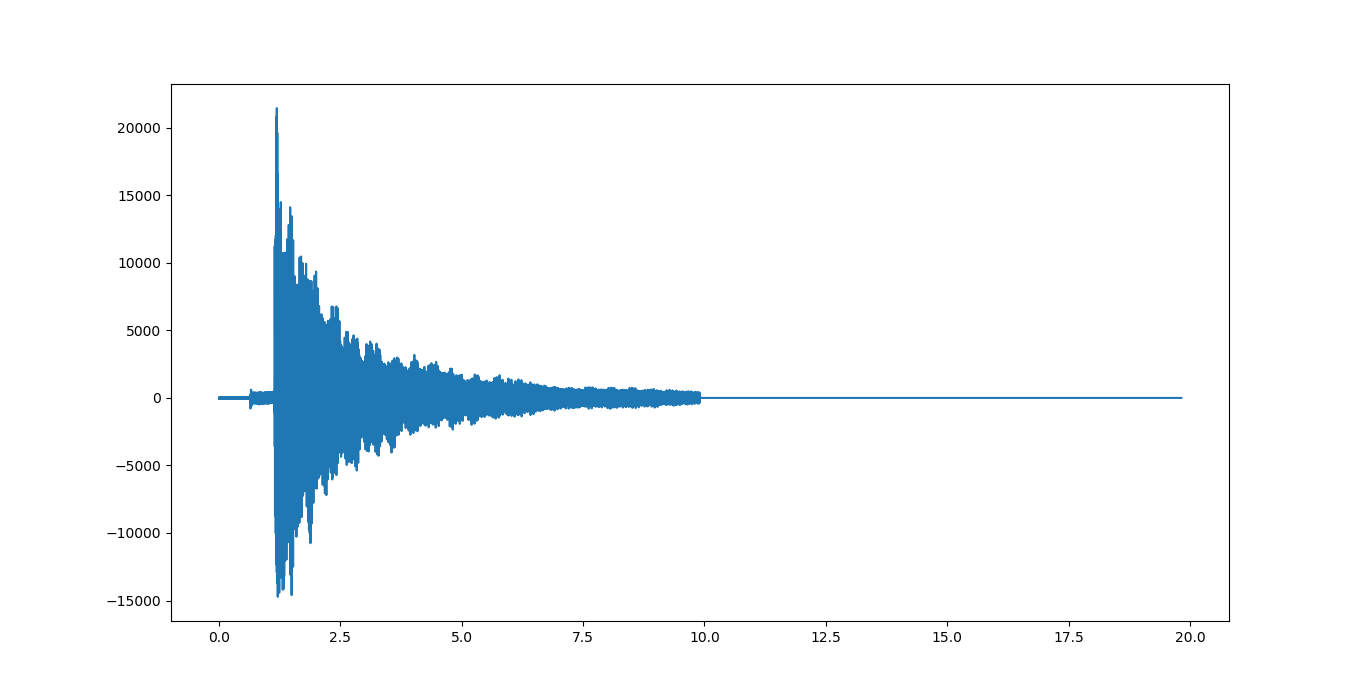
\includegraphics[width=\textwidth]{img/input-signal}
	\caption{An example of an input signal - in this case a $C_{maj}$ chord}
	\label{fig:input-signal}
\end{figure}

\paragraph*{}
The computer is instructed to load the amplitude samples of the signal in a 
column vector $A$.
$$A =
\begin{pmatrix}
	a \\
	b \\
	c \\
	d \\
	e \\
	\vdots
\end{pmatrix}\text{where, $a$, $b$, $c$, $d$ and $e$ are sample values}
$$
The \textit{Microsoft Waveform} datatype does not give information on the $x$ 
axis, as these values are inferred to be a linear space\footnote{A vector of 
linearly equidistant values} from $0$ to the norm of the $y$ vector. To get 
precise time information, ie. to get the number of seconds for every point in 
the $y$ vector, it is necessary to use the sampling frequency of the 
\textit{.wav} file. This sampling frequency, $F_s$, gives the number of samples
taken in a single second, ie. the number of $y$ values per single second. 
Finally, to get the values of the $x$ axis, it is necessary to multiply the 
aforementioned linear space by the reciprocal of the sampling frequency. The 
domain of the \textit{.wav} file is stored in the $t$ column vector:
$$t = \frac{1}{F_s} \cdot
\begin{pmatrix}
	0 \\
	1 \\
	2 \\
	3 \\
	\vdots
\end{pmatrix}\text{, where $|t| = |A|$}
$$
With these values, it is possible to proceed in the algorithm.

\subsection{The Fourier transformation}
A fast Fourier transformation\footnote{The fast Fourier transformation is a 
computer program implementation of the Fourier transformation which is faster
than the standard implementation of the Fourier transformation, but produces 
equal results. It utilizes functions exclusive to computer science.} is ran on 
the amplitude vector.
$$F = \text{fft(}t, A\text{)}$$
The Fourier transformation gives a symmetric vector of both positive and 
negative values, so the negative values are ignored, as their absolute values 
are equal to the positive ones, and they provide no relevant information.
$$F' =
\begin{pmatrix}
	F_1 \\
	F_2 \\
	F_3 \\
	\vdots \\
	F_{\frac{|F|}{2}}
\end{pmatrix}
$$
Since the numbers given by the Fourier transformation are complex, to get the 
amplitudes of the frequencies it is necessary to get absolute values for all 
of the values in the vector given by the Fourier transformation.
$$F'' = 
\begin{pmatrix}
	|F'_1| \\
	|F'_2| \\
	|F'_3| \\
	\vdots \\
	|F'_{|F'|}|
\end{pmatrix}
$$
A vector $f$ is created to store the domain of the Fourier transformation, 
such that it is a linear space from $0$ to $1$ with the norm being equal to 
the one returned Fourier transformation, multiplied by the sampling frequency 
of the original file. This is in turn, creates the frequency domain.
$$f = F_s \cdot
\begin{pmatrix}
	0 \\
	\vdots \\
	1
\end{pmatrix}\text{, such that $|f| = |F''|$}
$$

\subsection{Fourier transform peak identification} 
\paragraph*{}
In this section of the algorithm the computer tries to identify which peaks 
play a significant role in composing a chord. 

\paragraph*{} 
The vector $F''$ is normalized first:
$$F''' = \frac{1}{\text{max(}F''\text{)}} \cdot F''$$
This is useful for the next step, finding values that are bigger than a 
constant cutoff value $c_o$ and storing them in a vector $p$:
$$p = \varnothing$$
$$\forall v \in F''' : \bigg(v > c_o \Rightarrow p = 
	\begin{pmatrix}
		p \\
		v
\end{pmatrix} \bigg)$$
As an example, the normalized Fourier transformation, alongside the cutoff 
value of $c_o = 0.15$, is plotted in figure \ref{fig:fourier-signal}.
\begin{figure}[ht]
	\centering
	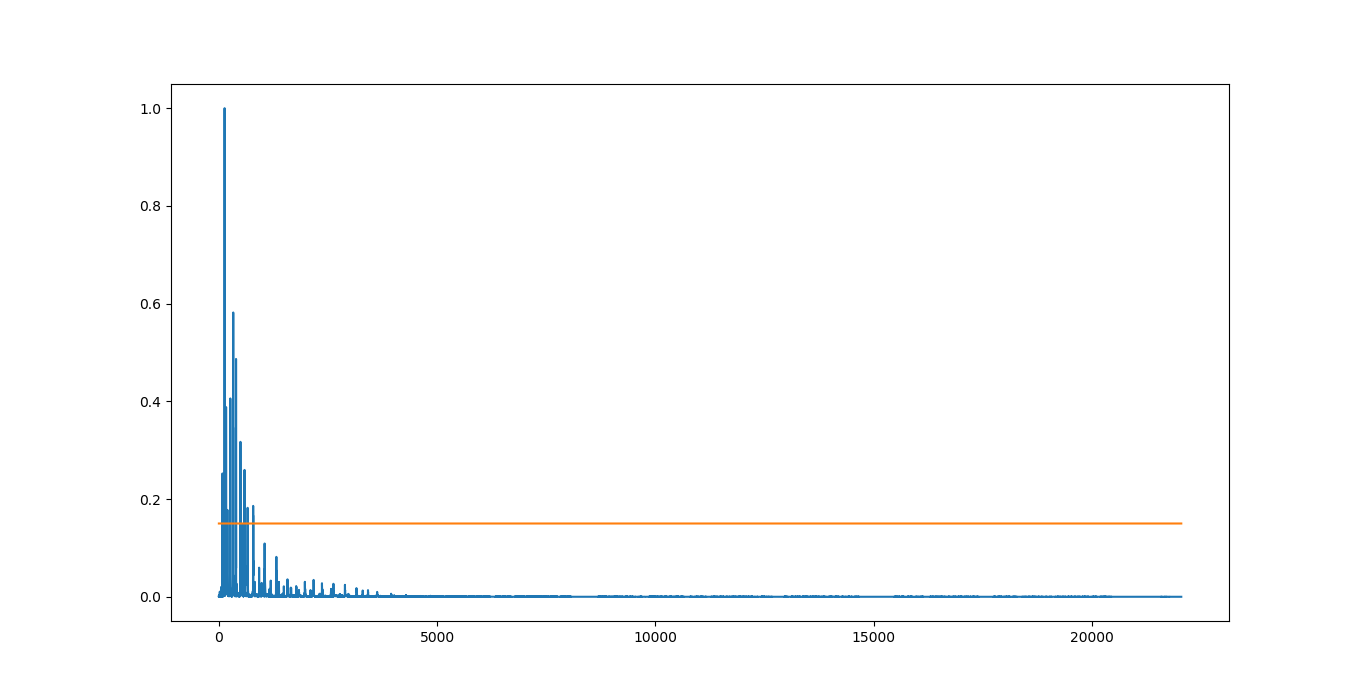
\includegraphics[width=\textwidth]{img/fourier-signal}
	\caption{The normalized Fourier transformation of the signal given in 
	figure \ref{fig:input-signal}, ie. a $C_{maj}$ chord.}
	\label{fig:fourier-signal}
\end{figure}

\paragraph*{} 
Note that the $p$ vector does not contain the individual frequencies of the 
notes played, but contains multiple values which resolve to one frequency, due 
to the fact that the Fourier transformation is a continuous function. To 
resolve this issue, the average of neighboring values is calculated. 
Neighboring values $w$ are neighboring to a value $v$ if the absolute 
difference between them is less than a leeway value $l$.
$$p' = \varnothing$$
$$\forall v \in p : \Bigg( 
	\bigg(\big(w \not\in p' : \abs{v - w} < l \big) \rightarrow p' = 
		\begin{pmatrix}
			p' \\
			w
		\end{pmatrix}
	\bigg) \land
	\bigg(\big(w \in p' : \abs{v - w} < l \big) \rightarrow
		w = (w + v) / 2
	\bigg)
\Bigg)$$
At this point, the vector $p'$ contains the frequencies of the played chord 
that are more intense than a given cutoff value.

\subsection{Note identification}
Notes are identified in this step by finding the closest value in a look-up 
table of frequencies\footnote{This table is available at the following link: 
\url{https://pages.mtu.edu/~suits/notefreqs.html}.}. As well as identifying 
the most plausible notes the certainty of a frequency being a single note is 
calculated according to the following. In this section, let us denote any 
value in $p'$ as $v$. Let us also denote the lookup table as a column vector 
$r$. We start from the premise that $v$ lies between two closest values in $r$:
$$r_n < v < r_{n+1}$$
First, we identify the closest value to $v$. At this point, we know either 
$r_n$ or $r_{n+1}$, but we do not know the other. To calculate the certainty 
of $v$ being the note $r_n$ or $r_{n+1}$ we need to calculate the unknown 
value. This is done with the following logical assertion. First denote the 
index of the known value ($r_n$ or $r_{n+1}$ as $k$). Next, calculate a value 
$o$ according to:
$$\Big((\abs{v - r_k} > \abs{v - r_{k+1}}) \Rightarrow o = r_{k+1} \land 
\neg (\abs{v - r_k} > \abs{v - r_{k+1}}) \Rightarrow o = r_{k-1}\Big)$$
Finally, calculate the certainty $c$ according to:
$$c = 1 - \frac{\abs{v - r_k}}{\abs{o - r_k}}$$

\subsection*{}
\paragraph*{}
The full algorithm is available at the following link: \url{}
%TODO Put the link

\subsection{Chord identification}
\paragraph*{}
Since this algorithm is only designed for chord triads, it was not difficult 
to design an algorithm which identifies chords from the previously identified 
notes. A simple look-up table was created and a simple searching algorithm was 
implemented.

\section{Evaluation}
\paragraph*{}
To identify how well the algorithm performs tests were created. $10$ guitar 
chord samples were downloaded from the internet (\textit{vide} the works 
cited). These chord samples were then analyzed using the algorithm. Since it 
was known which chords were played, it was possible to determine the accuracy 
of the algorithm.

\paragraph*{}
For a value of $c_o = 0.15$, the algorithm's success rate was $60\%$. However, 
when the value of $c_o$ was chosen to be a value greater or lesser than $0.15$ 
different success rates were achieved. A plot of the relationship between 
$c_o$ and the success rate of the algorithm is given in figure 
\ref{fig:success-rate}.
\begin{figure}[ht]
	\centering
	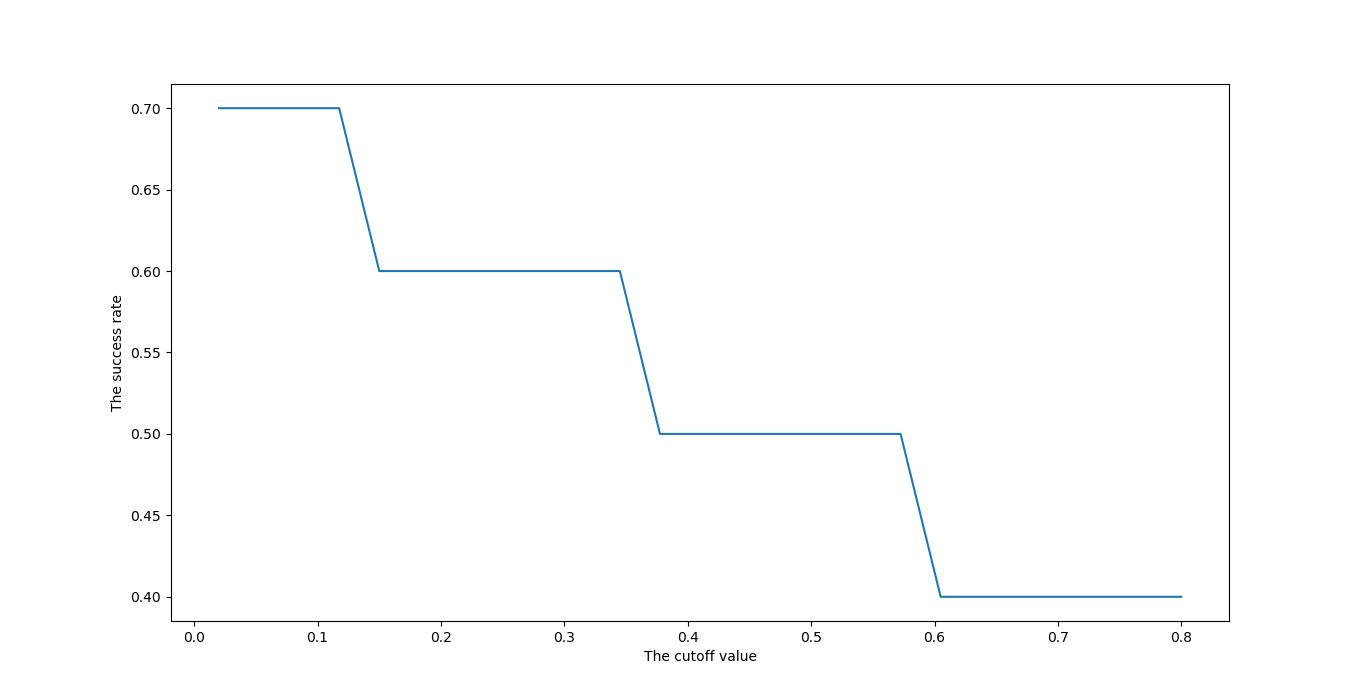
\includegraphics[width=\textwidth]{img/success-rate}
	\caption{The relationship between $c_o$ and the success rate of the 
	algorithm.}
	\label{fig:success-rate}
\end{figure}

\paragraph*{}
It is obvious that the maximal success rate is achieved for the minimal value 
of $c_o = 0.02$. This success rate is equal to $70\%$. Note, however, that 
the chords played in the samples might have not been the ones that the authors 
stated they were. It is possible that the guitars the chords were played on 
were out of tune, or the chords were played improperly, or the tune of the 
guitars was not one of $A_4 = 440$, or it is even possible that the guitars 
used were not precisely manufactured.

\section{Conclusion}
\paragraph*{}
The algorithm seems effective in achieving the required result. The evaluation 
of the algorithm was incomplete, due to a lack of chord samples. For more 
accurate evaluation it is necessary to use better chord samples.

\clearpage
\pagebreak
\section*{Works cited}
\begin{hangparas}{.25in}{1}

``A Minor Chord (Ringout)''. Freesound.Org, 2014, 
\url{https://freesound.org/people/dxe10/sounds/234061/}. Accessed 6 Oct 2018. \\

Benward, Bruce, and Marilyn Nadine Saker. 
\textit{Music In Theory And Practice}. Mcgraw-Hill, 2009. \\

``Frequencies Of Musical Notes, A4 = 440 Hz''. \textit{Pages.Mtu.Edu}, 2018, 
\url{https://pages.mtu.edu/~suits/notefreqs.html}. Accessed 3 Aug 2018. \\

``Guitar - Major Chords Pack''. Freesound.Org, 2018, 
\url{https://freesound.org/people/danglada/packs/1011/}. Accessed 6 Oct 2018. \\

Hausner, Christoph. \textit{``Design And Evaluation Of A Simple Chord 
Detection Algorithm''}. University Of Passau, 2014. \\

``Integral Over A Period Interval''. \textit{Planetmath.Org}, 2018, 
\url{http://planetmath.org/integraloveraperiodinterval}. Accessed 31 July 2018.
\\

Muludi, Kurnia, Aristoteles, and Abe Frank SFB Loupatty. \textit{``Chord 
Identification Using Pitch Class Profile Method With Fast Fourier Transform 
Feature Extraction''}. International Journal Of Computer Science Issues, vol 
11, no. 3, 2018, pp. 139-144. \\

Shazam Entertainment, Ltd. \textit{An Industrial-Strength Audio Search 
Algorithm}. 2018, 
\url{http://www.ee.columbia.edu/~dpwe/papers/Wang03-shazam.pdf}. 
Accessed 30 July 2018. \\

Valente, Michael et al. \textit{Audiology}. Thieme, 2008. \\

\end{hangparas}
\end{document}
